\subsection{Final selection}
\label{sec:eejjFinalSelection}
   
Table~\ref{tab:eejjFinalSelection} shows the number of events
for the data, the backgrounds, and the LQ signal, after applying the final, optimized \eejj~selection 
criteria summarized in Table~\ref{tab:eejjOptimizedCuts}.
Figures~\ref{fig:st_mej_fullSelection400_eejj} and~\ref{fig:st_mej_fullSelection600_eejj} show the 
distributions of \st~and the electron-jet invariant mass, \mej, for both leptoquark candidates (2 entries in for each event) after the full selection 
optimized for \MLQ$=400$ and 600~\GeV, respectively. 
The dominant background contributions are from \ttbar~and \zjets~events, 
while the contribution from the other backgrounds is below \OtherBackgroundContributionINeejj~for 
the LQ masses within the current reach of this analysis. 
A good agreement is observed between the data and the background 
prediction within statistical uncertainties.    

\begin{table} 
\small 
\begin{tabular}{l | c | c | c | c | c | c | c } 
$M_{LQ}$ & LQ Signal & Z+Jets & $t\bar{t}$ & QCD & Other & Data &  Total BG \\ 
  \hline 
  \hline 
Presel & -                   &  $ 6234 \pm 24 $   & $ 768 \pm 19 $        & $ 49.59 \pm 0.43 $       & $ 147.6 \pm 2.3 $ &7201 & $ 7199 \pm 31 $ \\ 
  \hline 
250 &  $ 6846.2 \pm 32.0 $   &  $ 385 \pm 6.0 $   & $ 334 \pm 13 $        & $ 17.726 \pm 0.186 $     & $ 28.3 \pm 1.3  $ &770 & $ 765 \pm 14 $ \\ 
350 &  $ 1119.6 \pm 4.5 $    &  $ 88.5 \pm 2.8 $  & $ 41.2 \pm 4.5 $      & $ 1.934 \pm 0.034 $      & $ 6.11 \pm 0.64 $ &139 & $ 138 \pm 5.4 $ \\ 
400 &  $ 487.4 \pm 2.2 $     &  $ 35.7 \pm 1.8 $  & $ 19.1 \pm 3.1 $      & $ 0.877 \pm 0.022 $      & $ 3.12 \pm 0.56 $ &55  & $ 58.8 \pm 3.6 $ \\ 
450 &  $ 225.6 \pm 1.0 $     &  $ 15.2 \pm 1.1 $  & $ 7.8 \pm 2.0 $       & $ 0.310 \pm 0.013 $      & $ 1.92 \pm 0.60 $ &26  & $ 25.2 \pm 2.3 $ \\ 
500 &  $ 109.30 \pm 0.46 $   &  $ 6.55 \pm 0.70 $ & $ 2.45 \pm 1.10 $     & $ 0.192 \pm 0.012 $      & $ 1.03 \pm 0.42 $ &14  & $ 10.2 \pm 1.4 $ \\ 
550 &  $ 57.35 \pm 0.23 $    &  $ 4.65 \pm 0.58 $ & $ 0.98 \pm 0.69 $     & $ 0.139 \pm 0.012 $      & $ 0.84 \pm 0.42 $ &11  & $ 6.60 \pm 0.99 $ \\ 
600 &  $ 30.95 \pm 0.14 $    &  $ 3.04 \pm 0.46 $ & $ 0.49 \pm 0.49 $     & $ 0.088 \pm 0.011 $      & $ 0.72 \pm 0.41 $ &8   & $ 4.34 \pm 0.79 $ \\ 
650 &  $ 16.998 \pm 0.0647 $ &  $ 2.14 \pm 0.38 $ & $ 0.49 \pm 0.49 $     & $ 0.073 \pm 0.011 $      & $ 0.48 \pm 0.40 $ &6   & $ 3.18 \pm 0.74 $ \\ 
750 &  $ 5.5264 \pm 0.0230 $ &  $ 1.04 \pm 0.26 $ & $ 0.00_{-0.00}^{+0.56}$ &  $ 0.00923 \pm 0.00203 $ & $ 0.41 \pm 0.40 $ &0   & $ 1.453_{-0.47}^{+0.73}$ \\ 
850 &  $ 1.9679 \pm 0.0078 $ &  $ 0.81 \pm 0.23 $ & $ 0.00_{-0.00}^{+0.56}$ &  $ 0.00101 \pm 0.00022 $ & $ 0.40 \pm 0.40 $ &0   & $ 1.21_{-0.46}^{+0.72}$ \\ 
900 &  $ 1.1968 \pm 0.0044 $ &  $ 0.81 \pm 0.23 $ & $ 0.00_{-0.00}^{+0.56}$ &  $ 0.00101 \pm 0.00022 $ & $ 0.40 \pm 0.40 $ &0   & $ 1.21_{-0.46}^{+0.72}$ \\ 
\end{tabular}
\caption{Number of events after the final \eejj~selection. Only statistical uncertainties are reported.}
\label{tab:eejjFinalSelection}
\end{table}


\begin{figure}[htbp]
  \begin{center}
    \begin{tabular}{cc}
      \resizebox{7.5cm}{!}{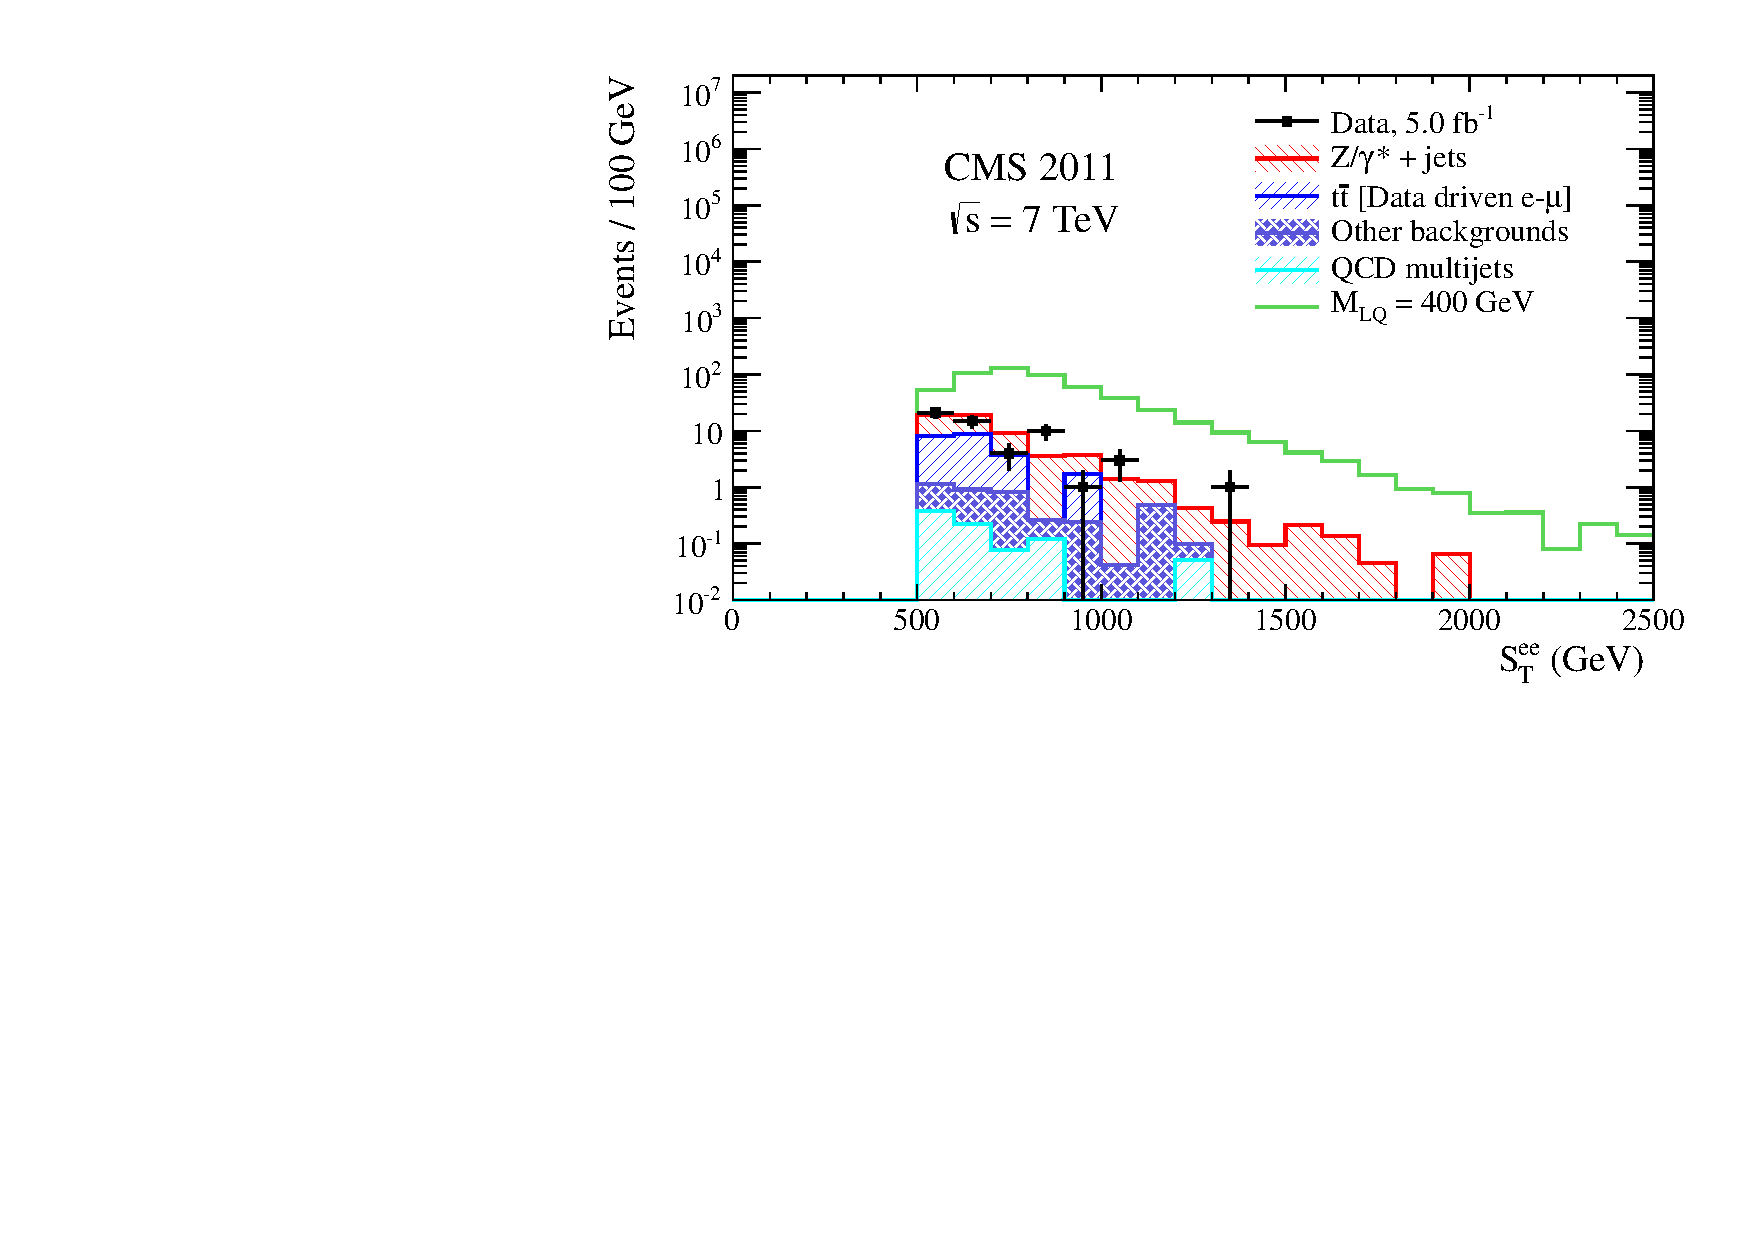
\includegraphics{tex/analysis/event_selection/fig/ee/final_selection/sT_eejj_LQ400_eejj_WZSherpa.pdf}} &
      \resizebox{7.5cm}{!}{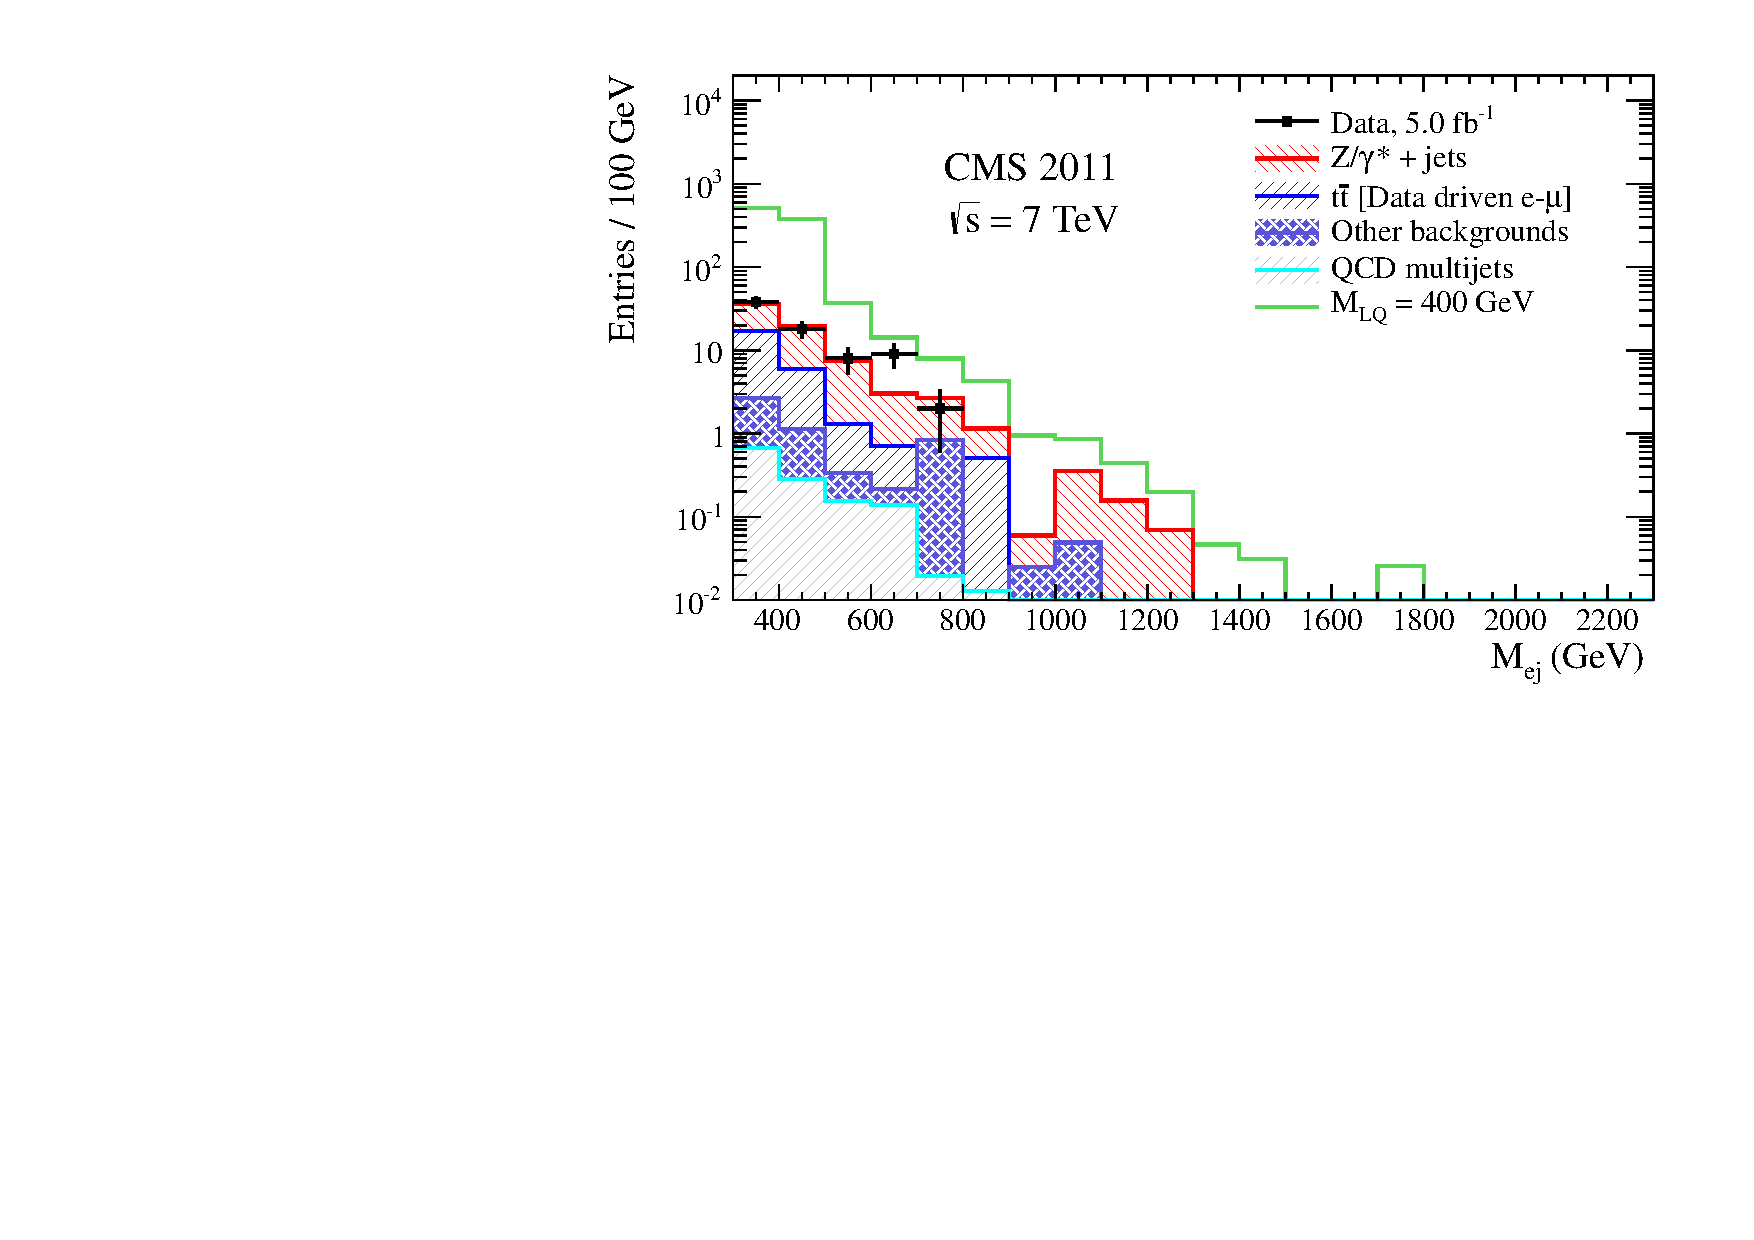
\includegraphics{tex/analysis/event_selection/fig/ee/final_selection/Mej_minmax_LQ400_eejj_WZSherpa.pdf}} \\
    \end{tabular}
    \caption{The \st~(left)
             and \mej~(right) distributions 
             for events passing the full \eejj~selection optimized for \MLQ$=400$~\GeV.
             The \mej~distribution on the right has two entries per event: one for each
             leptoquark candidate.
    }
    \label{fig:st_mej_fullSelection400_eejj}
  \end{center}
\end{figure}

\begin{figure}[htbp]
  \begin{center}
    \begin{tabular}{cc}
      \resizebox{7.5cm}{!}{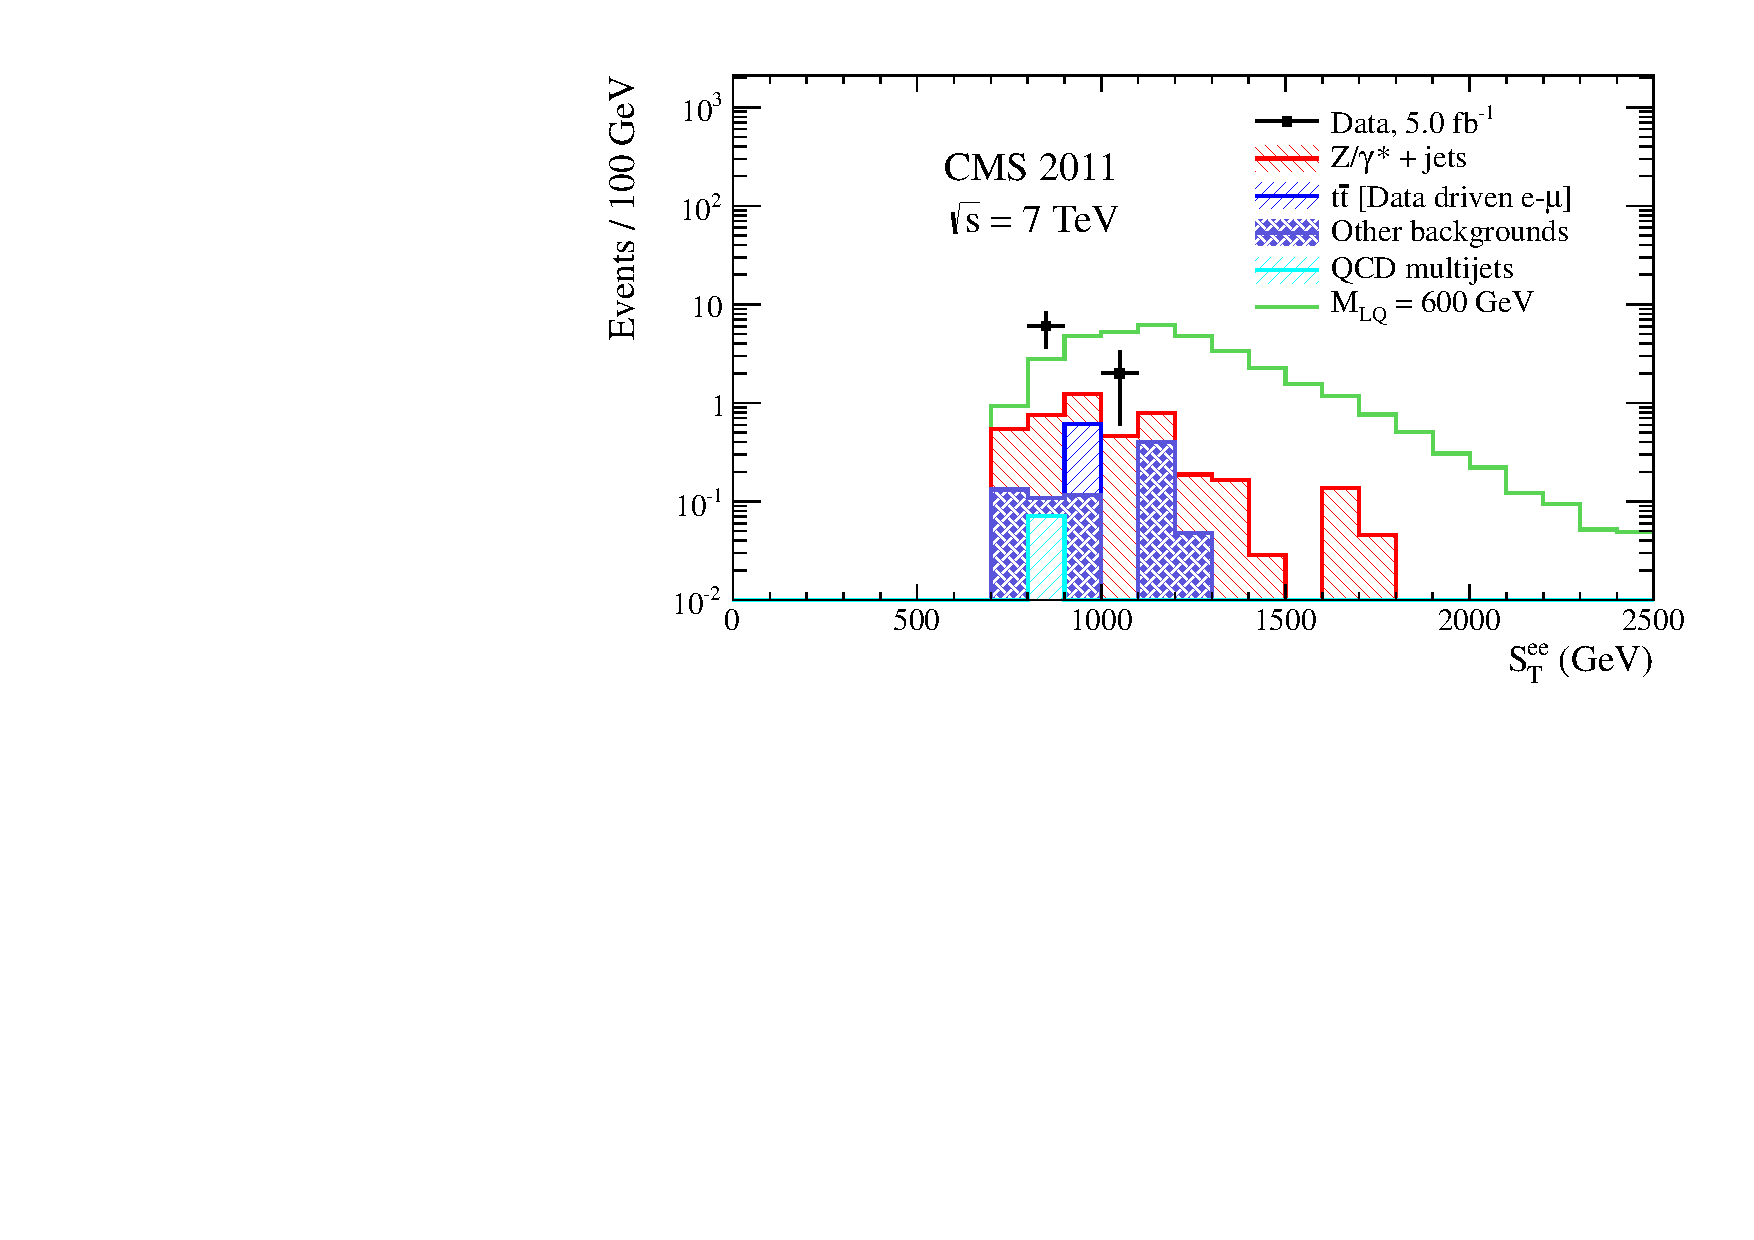
\includegraphics{tex/analysis/event_selection/fig/ee/final_selection/sT_eejj_LQ600_eejj_WZSherpa.pdf}} &
      \resizebox{7.5cm}{!}{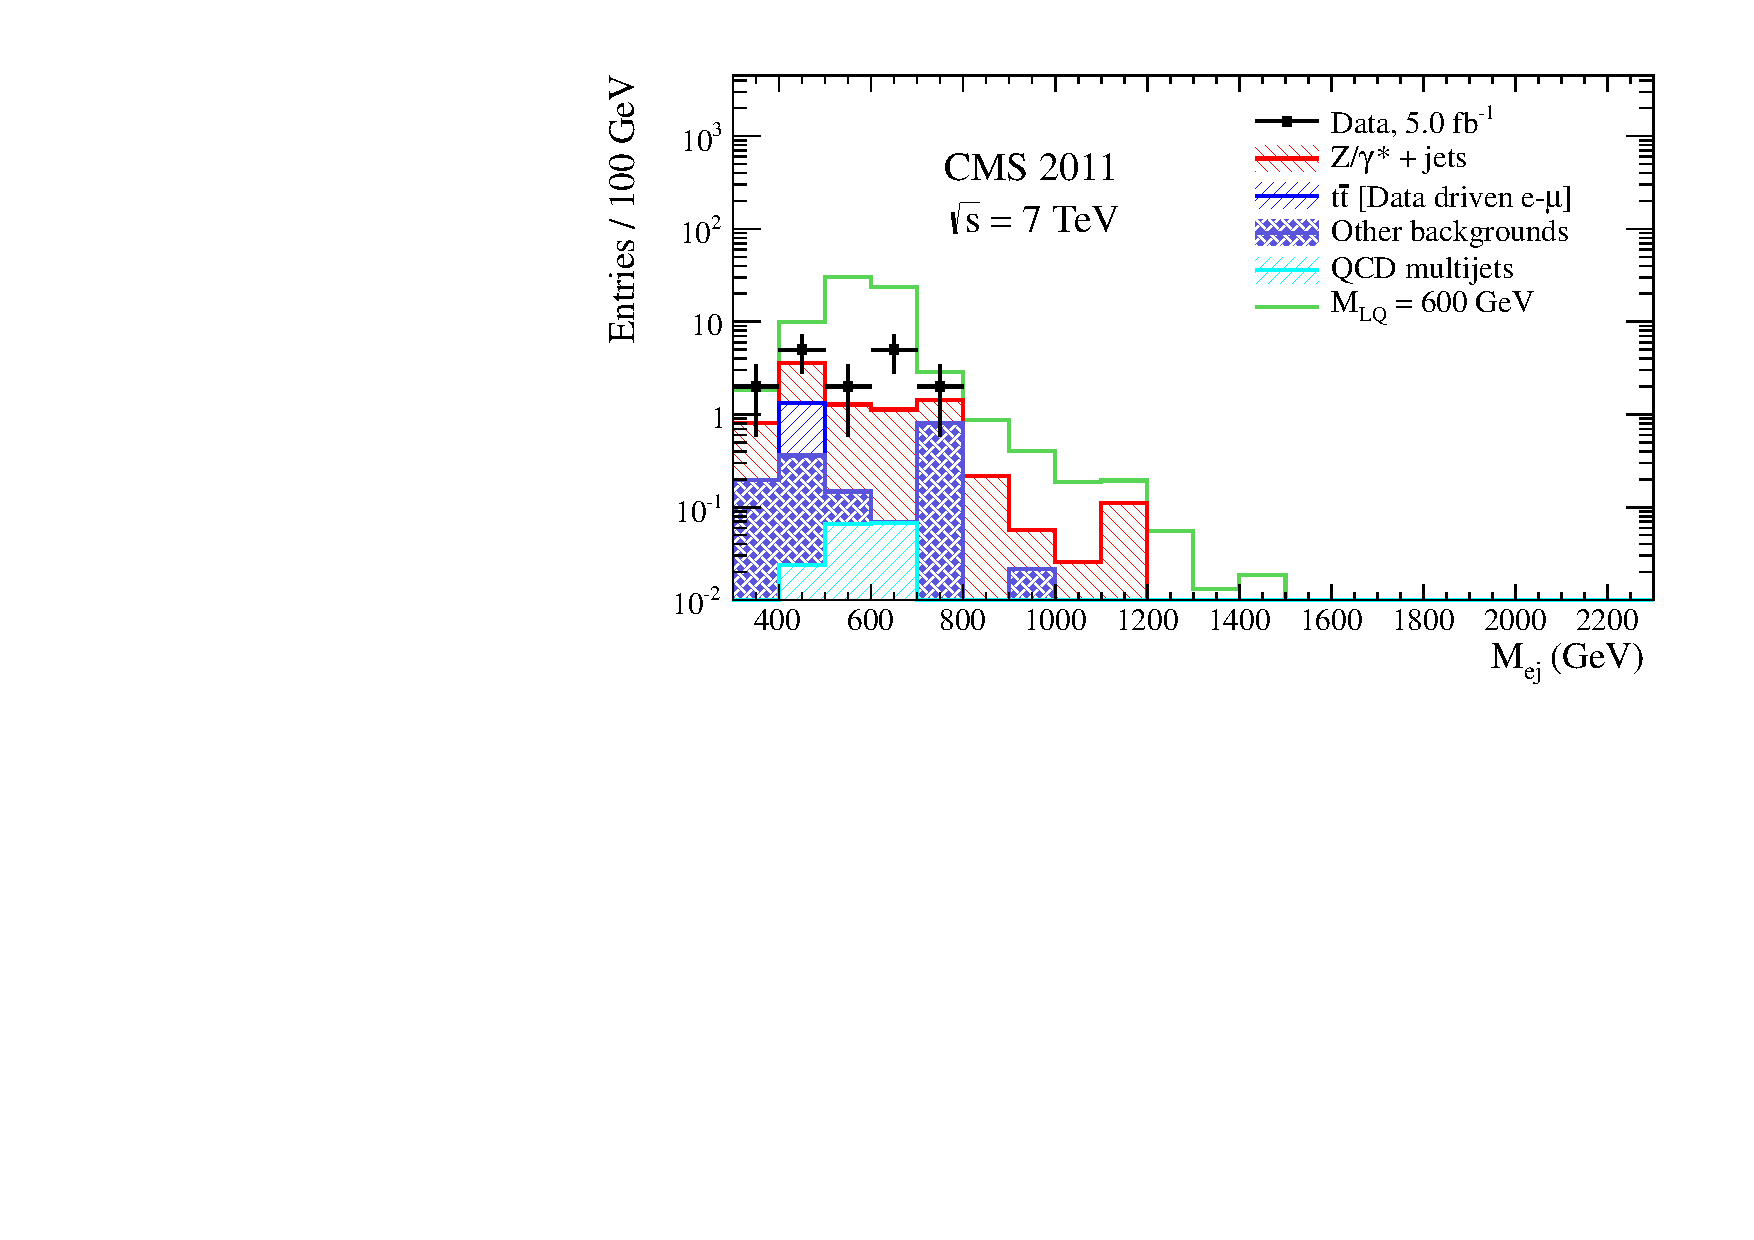
\includegraphics{tex/analysis/event_selection/fig/ee/final_selection/Mej_minmax_LQ600_eejj_WZSherpa.pdf}} \\
    \end{tabular}
    \caption{The \st~(left)
             and \mej~(right) distributions 
             for events passing the full \eejj~selection optimized for \MLQ$=600$~\GeV.
             The \mej~distribution on the right has two entries per event: one for each
             leptoquark candidate.
    }
    \label{fig:st_mej_fullSelection600_eejj}
  \end{center}
\end{figure}
